%!mode::"TeX:UTF-8"
\documentclass{ctexart}
\usepackage{amsmath}
\usepackage{amssymb}
\usepackage{xltxtra}
\usepackage{mflogo,texnames}
\usepackage{graphicx}
\usepackage{listings}
\usepackage{listing}
\usepackage{xcolor}
\usepackage{xcolor}
\usepackage{enumerate}
\usepackage[colorlinks,linkcolor=blue]{hyperref}
\usepackage{cite}
\usepackage{color}
\usepackage{caption}
\usepackage{subfigure}
\usepackage[top=2.54cm,bottom=2.54cm,left=3.18cm,right=3.18cm]{geometry}
\author{右武卫大将军}
\title{序列建模:循环和递归网络}
\begin{document}
    \maketitle
    循环网络(RNN)是一类用于处理序列数据的神经网络。就像卷积网络是用于处理网格化数据的神经网络,循环神经网络是用于处理序列$x^{(1)},\cdots,x^{(n)}$的神经网络。正如卷积网络可以很容易地拓展到具有很大宽度和高度的图像,以及处理大小可变的图像,循环神经网络可以拓展到更长的序列(比不基于序列的特化网络长得多)。大多数循环网络也能处理可变长度的序列。

    从多层网络出发到循环网络,我们需要利用20世纪80年代机器学习和统计模型早期思想的优点:在模型的不同部分共享参数。参数共享使得模型能够拓展到不同形式的样本({\color{red} 这里指长度不同的样本})并进行泛化。如果我们在每一个时间点都有单独的参数,不但不能泛化到训练时没有见过的序列长度,也不能在时间上共享不同序列长度和不同位置的统计强度。当信息的特定部分会在序列内多个位置出现时,这样的共享尤为重要。例如,考虑这两句话:“I went to Nepal in 2009”和“In 2009,I went to Nepal”。 如果我们让一个机器学习模型读取这两个句子,并提取叙述者去Nepal的年份,无论“2009年”作为句子的第六个单词还是第二个单词出现,我们都希望模型能认出“2009年”作为相关资料片段。假设我们要训练一个处理固定长度句子的前馈网络。传统的全连接前馈网络会给每个输入特征分配一个单独的参数,所以需要分别学习句子每个位置的所有语言规则。相比之下,循环神经网络在几个时间步内共享相同的权重,不需要分别学习句子每个位置的所有语言规则。

    一个相关的想法是在一维时间序列上使用卷积。这种卷积方法是时延神经网络的基础。卷积操作允许网络跨时间共享参数,但是浅层的。卷积的输出是一个序列,其中输出中的每一项是相邻几项输入的函数。参数共享的概念体现在每一个时间步中使用的相同的卷积核。循环神经网络以不同的方式共享参数。输出的每一项是前一项的函数。输出的每一项对先前的输出应用应用相同的更新规则而产生。这种循环方式导致参数通过很深的计算图共享。

    为了简单起见,我们说的RNN是指在序列上的操作,并且该序列在时刻$t$(从1到$\tau$)包含向量$x^{(t)}$。在实际情况上,循环网络通常在序列的小批量上操作,并且小批量的每项具有不同序列长度$\tau$。我们省略小批量索引来简化记号。此外,时间步索引不必是字面上现实世界中流逝的时间。有时,它仅表示序列中的位置。RNN也可以应用于跨越两个维度的空间数据(如图像)。当应用于涉及时间的数据,并且将整个序列提供给网络之前就能观察到整个序列时,该网络可具有关于时间向后的连接。

    本章将计算图的思想拓展到包括循环。这些周期代表变量自身的值在未来某一时间步对自身值的影响。这样的计算图允许我们定义循环神经网络。然后,我们描述许多构建,训练和使用循环神经网络的不同方式。

    本章将要简要介绍循环神经网络。

    \section{展开计算图}
        计算图是形式化一组计算结构的方式,如那些涉及将输入和参数映射到输出和损失的计算。本节,我们对展开(unfolding)递归或者循环计算得到的重复结构进行解释,这些重复结构通常对应于一个事件链。展开这个计算图将导致深度网络结构中的参数共享。

        例如,考虑动态系统的经典形式:
        \begin{equation}
            s^{(t)} = f(s^{(t-1)};\theta)
            \label{e10.1}
        \end{equation}
        其中$s^{(t)}$称为系统的状态。

        $s$在时刻$t$的定义需要参考时刻$t-1$时同样的定义,因此\ref{e10.1}是循环的。

        对有限时间步$\tau,\tau-1$次应用这个定义可以展开这个图。例如$\tau=3$,我们对\ref{e10.1}展开,可以得到
        \begin{equation}
            \begin{split}
                s^{(3)} &= f(s^{(2)};\theta) \\
                        &= f(f(s^{(1)};\theta);\theta)
            \end{split}
            \label{e10.3}
        \end{equation}
        以这种方式重复应用定义,展开等式,就能得到不涉及循环的表达式。现在我们可以使用传统的有向无环图呈现这种的表达。

        式子\ref{e10.3}所展开的计算图如图\ref{f10.1}所示。
        \begin{figure}[hb]
            \centering
            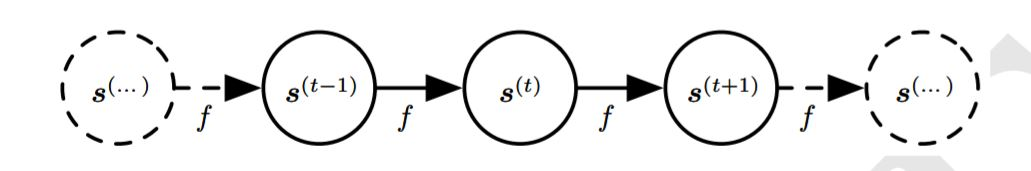
\includegraphics[width=0.7\textwidth]{f1}
            \caption{将经典的动态系统展示为展开的计算图。每一个节点表示在某个时刻$t$的状态,并且函数$f$将$t$处的状态映射到$t+1$处的状态。所有时间步都使用相同的参数}
            \label{f10.1}
        \end{figure}
        作为另一个例子,让我们考虑由外部信号$x^{(t)}$驱动的动态系统,
        \begin{equation}
            s^{(t)} = f(s^{(t-1)},x^{(t)};\theta)
            \label{e10.4}
        \end{equation}
        我们可以看到,当前的状态包含整个过去序列的信息。

        循环网络可以通过许多不同的方式建立。就像几乎所有函数都可以被认为是前馈网络,本质上任何涉及循环的函数都可以视为循环神经网络。

        很多循环网络使用公式\ref{e10.5}或类似的公式定义隐藏单元的值。为了表明状态是网络的隐藏单元,我们使用变量$h$代表状态重新\ref{e10.4}:
        \begin{equation}
            h^{(t)} = f(h^{(t-1)},x^{(t)};\theta)
            \label{e10.5}
        \end{equation}
        如图\ref{f10.2}所示,典型RNN会增加额外的架构特性,如读取状态信息$h$作为预测的输出层。
        \begin{figure}
            \centering
            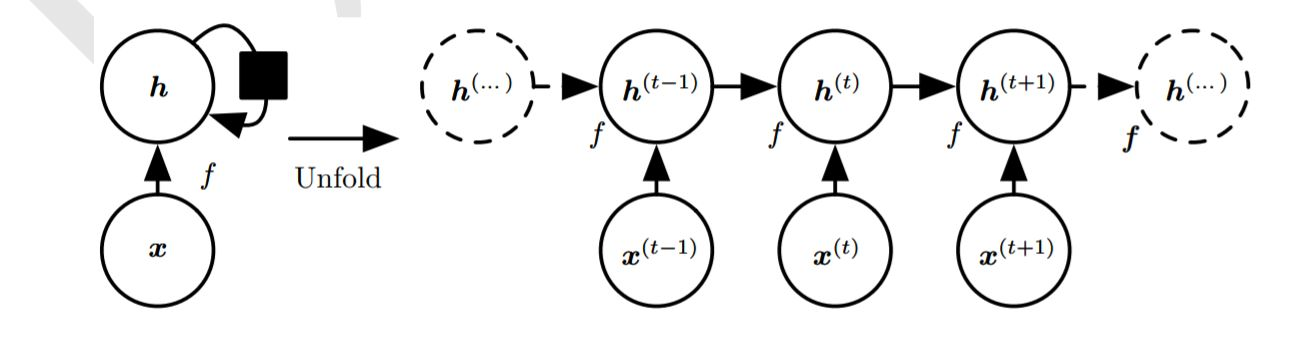
\includegraphics[width=0.7\textwidth]{f2}
            \caption{没有输出的循环网络。此循环网络只处理来自输入$x$的信息,将其合并到经过时间向前传播的状态$h$。(左)回路原理图。黑色方块表示单个时间步的延迟。(右)同一网络被视为展开的计算图,其中每个节点现在与一个特定的时间实例相关联}
            \label{f10.2}
        \end{figure}
        当训练循环网络根据过去预测未来时,网络通常要学会使用$h^{(t)}$作为过去序列与任务相关方面的有损摘要。此摘要一般而言一定是有损的,因为其映射任意长度的序列$(x^{(t)},x^{(t-1)},\cdots,x^{(2)},x^{(1)})$到一固定长度的向量$h^{(t)}$。根据不同的训练准则,摘要可能选择性地保留过去序列的某些方面。例如,如果在统计语言建模中使用的RNN,通常给定前一个词预测下一个词,可能没有必要存储时刻$t$前输入序列中的所有信息;而仅仅存储足够预测句子其余部分的信息。最苛刻的情况是,我们要求$h^{(t)}$足够丰富,并能大致恢复输入序列,如自编码框架。

        公式\ref{e10.5}可以使用不同的两种方式绘制。一种方法是为可能在模型的物理实现中存在的部分赋予一个节点,如生物神经网络。在这个观点下,网络定义了实时操作的回路,如图\ref{f10.2}左侧,其当前状态可以影响其未来的状态。在本章中,我们使用回路图的黑色方块表明在时刻$t$的状态到时刻$t+1$的状态单个时刻延迟中的相互作用。另一个绘制RNN的方法是展开的计算图,其中每一个组件由许多不同的变量表示,每一个时间步一个变量,表示在该时间点组件的状态。每一个时间步的每一个变量绘制为计算图的一个独立节点,如图\ref{f10.2}右侧所示。我们所说的展开是将左图中的回路映射为右图中包含重复组件的计算图的操作。目前,展开图的长度取决于序列的长度。

        我们用一个函数$g^{(t)}$代表经$t$步展开后的循环:
        \begin{equation}
            h^{(t)} = g^{(t)}(x^{(t)},x^{(t-1)},\cdots,x^{(2)},x^{(1)}) = f(h^{(t-1)},x^{(t)};\theta)
            \label{f10.7}
        \end{equation}
        函数$g^{(t)}$将全部的过去序列作为输入来生成当前的状态,但是展开的循环架构允许我们将它分解为函数$f$的重复应用,因此,展开过程引入了两个主要优点:

        (1)无论序列的长度,学习模型始终有相同的输入大小,因为它指定的是从一种状态到另一种状态的转移,而不是在可变长度的历史状态上操作。

        (2)我们可以在每个时间步使用相同参数的相同转移函数$f$。

        这两个因素使得学习在所有时间步和所有序列长度上操作单一模型是可能的。而不需要再所有可能时间步学习独立的模型$g^{(t)}$。学习单一的共享模型允许泛化到没有见过的序列长度,并且估计模型所需的训练样本远远少于不带参数共享的模型。

        无论是循环图还是展开图,都有其用途。循环图简洁。展开图能够明确描述其中的计算流程。展开图还通过显示的信息流动路径帮助说明信息在时间上向前(计算输出和损失)和向后(计算梯度)的思想。

    \section{循环神经网络}
        基于第一节中图展开和参数共享的思想,我们可以设计各种循环神经网络。

        循环神经网络中一些重要的设计模式包括以下几种:

        (1)每一个时间步都有输出,并且隐藏单元之间有循环连接的循环网络,如图\ref{f10.3}所示。
        \begin{figure}[h]
            \centering
            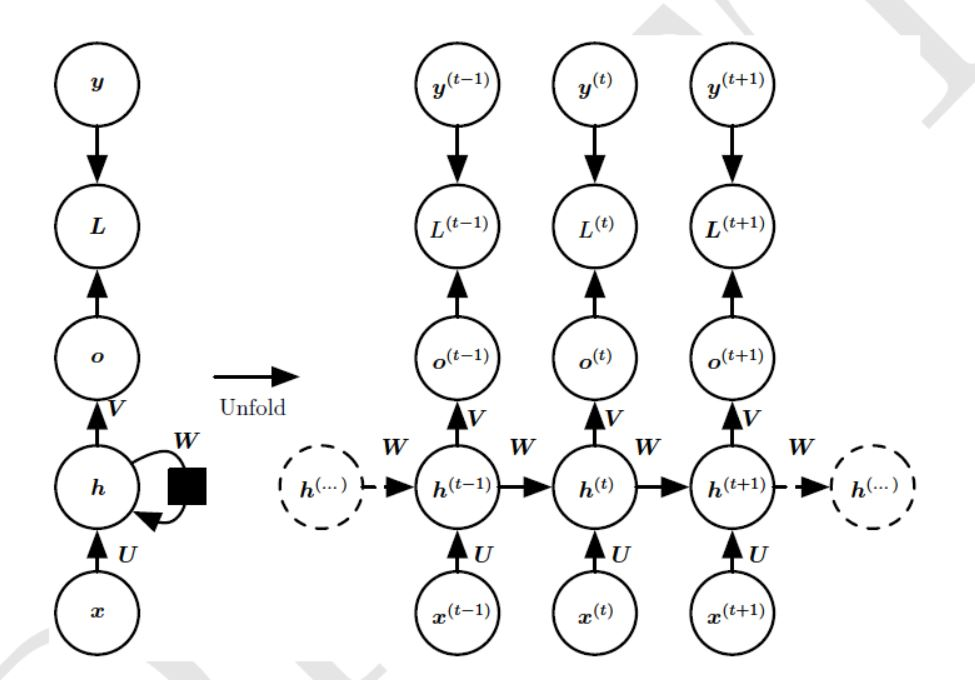
\includegraphics[width=0.9\textwidth]{f3}
            \caption{计算循环网络训练损失的计算图。损失$L$衡量每个$o$与相应的训练目标$y$的距离。当使用softmax输出时,我们假设$o$是未归一化的对数概率。损失$L$内部计算$\hat{y}=softmax(o)$,并将其与目标$y$ 比较。RNN输入到隐藏的连接由权重矩阵$U$参数化,隐藏到隐藏的循环连接由权重矩阵$W$参数化,以及隐藏到输出的连接由权重矩阵$V$参数化。式子\ref{e10.8}定义了该模型的前向传播。(左)使用循环连接绘制的RNN及其损失。(右)同一个网络被视为展开的计算图,每一个节点现在与特定的时间实例相关联}
            \label{f10.3}
        \end{figure}

        (2)每一个时间步都产生一个输出,只有当前时刻的输出到下个时刻的隐藏单元之间有循环连接的循环网络,如图\ref{f10.4}所示。
        \begin{figure}
            \centering
            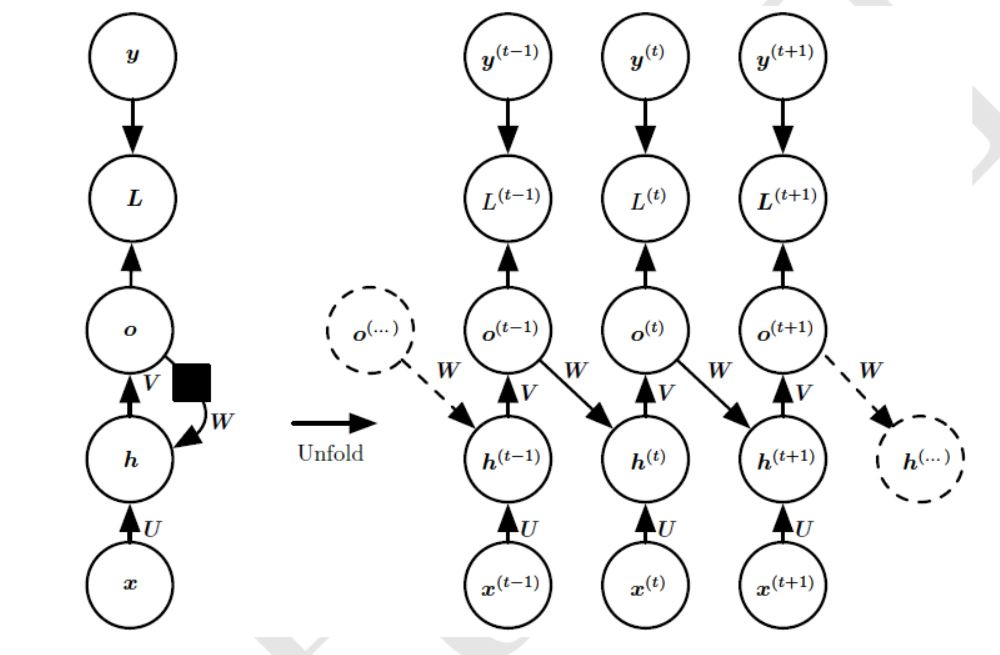
\includegraphics[width=0.9\textwidth]{f4}
            \caption{此类RNN的唯一循环是从输出层到隐藏层的反馈连接。在每个时间步$t$,输入为$x_t$,隐藏层激活为$h^{(t)}$,输出为$o^{(t)}$,目标为$y^{(t)}$,损失为$L^{(t)}$。(左)回路原理图。(右)展开的计算图。这样的RNN没有图\ref{f10.3}表示的RNN那样强大(只能表示更小的函数集合)。图\ref{f10.3}中的RNN可以选择将想要的关于过去的任何信息放入隐藏表示$h$中并且将$h$传播到未来。该图中的RNN被训练为将特定输出值放入$o$中,并且$o$是允许传播到未来的唯一信息。此处没有从$h$前向传播的直接连接。之前的$h$仅仅通过产生的预测间接的连接到当前。$o$通常缺乏过去的重要信息,除非它非常高维。这使得该图中的RNN不那么强大,但是它更容易训练,因为每一个时间步可以与其他时间步分离训练,允许训练期间更多的并行化}
            \label{f10.4}
        \end{figure}

        (3)隐藏单元之间存在循环连接,但是读取整个序列后产生单个输出的循环网络,如图\ref{f10.5}所示。
        \begin{figure}
            \centering
            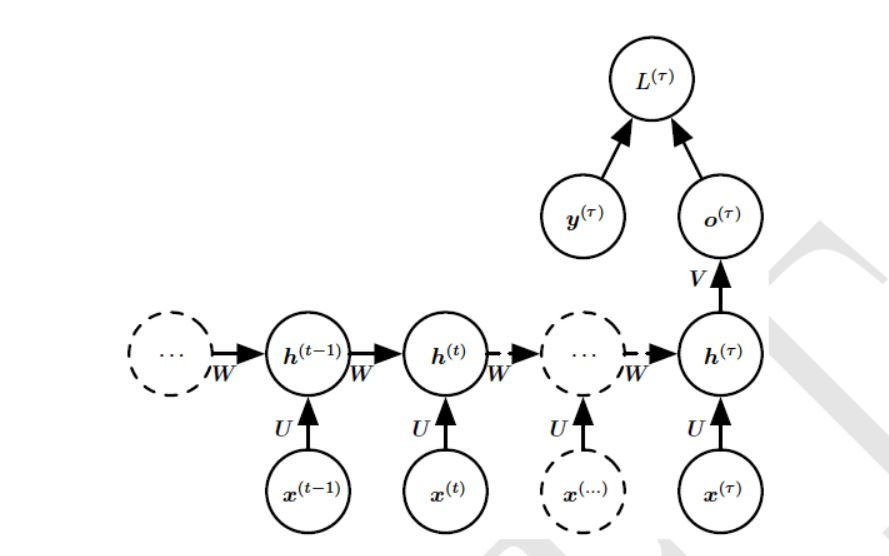
\includegraphics[width=0.9\textwidth]{f5}
            \caption{关于时间展开的循环神经网络,在序列结束时具有单个输出,这样的网络可以用于概括序列并产生用于进一步处理的固定大小的表示。在结束处可能存在目标,或者通过更下流模块的反向传播来获得输出$o^{(t)}$上的梯度}
            \label{f10.5}
        \end{figure}

        任何图灵可计算的函数都可以通过这样一个有限维的循环网络计算,在这个意义上图\ref{f10.3}和公式\ref{e10.8}的循环网络是万能的。RNN经过若干时间步后读取输出,这与由图灵机所用时间步是渐进线性的,与输入长度也是渐进线性的。由图灵机计算的函数是离散的,所以这些结果都是函数的具体实现,而不是近似。RNN作为图灵机使用时,需要一个二进制序列作为输入,其输出必须离散化以提供二进制输出。利用单个有限大小的特定RNN计算在此设置下的所有函数是可能的。图灵机的输入是要计算函数的详细说明,所以模拟此图灵机的相同网络足以应付所有问题。用于证明的理论RNN可以通过激活和权重来模拟无限堆栈。

        现在我们研究图\ref{f10.3}中RNN的前向传播公式。这个图没有指定隐藏单元。假设使用双曲正切函数。此外,图中没有明确指定何种形式的输出和损失函数。假定输出是离散的,如用于预测词或者字符的RNN。表示离散变量的常规方式是把输出$o$作为每个离散变量可能值的非标准化对数概率。然后,我们可以应用softmax函数后续处理后,获得标准化后概率的输出向量$\hat{y}$。RNN从特定的初始状态$h$开始前向传播。从$t=1$到$t=\tau$的每一个时间步,我们应用以下的更新方程:
        \begin{equation}
            \begin{split}
                a^{(t)} &= b + Wh^{(t-1)} + U x^{(t)} \\
                h^{(t)} &= tanh(a^{(t)}) \\
                o^{(t)} &= c + Vh^{(t)} \\
                \hat{y}^{(t)} &= softmax(o^{(t)})
            \end{split}
            \label{e10.8}
        \end{equation}
        其中参数的偏置向量$b$和$c$连同权重矩阵$U,V,W$,分别对应于输入到隐藏、隐藏到输出和隐藏到隐藏的连接矩阵。这个循环网络将一个输入序列映射到相同长度的输出序列。与$x$序列配对的$y$的总损失就是所有时间步的损失之和。例如,$L^{(t)}$为给定的$x^{(1)},\cdots,x^{(t)}$后$y^{(t)}$的负对数似然,则
        \begin{equation}
            L(\{x^{(1)},\cdots,x^{(t)}\},\{y^{(1)},\cdots,y^{(t)}\}) = \sum_t L^{(t)} = - \sum_t \log P_{model} (y^{(t)}|\{x^{(1)},\cdots,x^{(t)}\})
            \label{e10.12}
        \end{equation}
        关于各个参数计算这个损失函数的梯度是计算成本很高的操作,梯度计算涉及执行一次前向传播,接着是由右向左的反向传播,运行时间是$\mathcal{O}(\tau)$,并且不能通过并行化来降低,因为前向传播图是固有循序的:每一个时间步只能一前一后地计算。前向传播中的各个状态必须保持,直到他们反向传播中被再次使用,因此内存代价也是$\mathcal{O}(\tau)$。应用于展开图且代价为$\mathcal{O}(\tau)$的反向传播算法称为\textbf{通过时间反向传播}。因此隐藏单元之间存在循环的网络非常强大,但是训练代价也很大。我们是否有其他选择呢?
        \subsection{导师驱动过程和输出循环网络}
            仅在一个时间步的输出和下一时间步的隐藏单元之间存在循环连接的网络确实没有那么强大(因为缺乏隐藏到隐藏的循环连接)。例如,它不能模拟通用图灵机。因为这个网络缺少隐藏到隐藏的循环,它要求输出单元捕捉预测未来的关于过去的所有信息。因为输出单元明确地训练成匹配训练集的目标,它们不太能捕获关于过去输入历史的必要信息,除非用户知道如何描述系统的全部状态,并将它作为训练目标的一部分。消除隐藏到隐藏循环的优点在于,任何基于比较时刻$t$的预测和时刻$t$的训练目标的损失函数中的所有时间步都是解耦的。因此训练可以并行化,即在时刻$t$分别计算梯度。因为训练集提供输出的理想值,所以没有必要先计算出前一时刻的输出。

            由输出反馈到模型而产生循环链接的模型可用\textbf{导师驱动过程(teacher forcing)}进行训练。训练模型时,导师驱动过程不再使用最大似然准则,而在时刻$t+1$接受真实值$y^{(t)}$作为输入。我们可以通过检查两个时间步的序列得知这一点。条件最大似然准则是:
            \begin{equation}
                \log P(y^{(1)},y^{(2)}|x^{(1)},x^{(2)}) = \log P(y^{(2)}|y^{(1)},x^{(1)},x^{(2)}) + \log P(y^{(1)}|x^{(1)},x^{(2)})
                \label{e10.15}
            \end{equation}
            在这个例子中,同时给定迄今为止的$x$序列和来自训练集的前一个$y$值,我们可以看到在时刻$t=2$时,模型被训练为最大化$y^{(2)}$的条件概率。因此最大似然在训练时指定正确反馈,而不是将自己的输出反馈到模型,如图\ref{f10.6}所示。
            \begin{figure}[h]
                \centering
                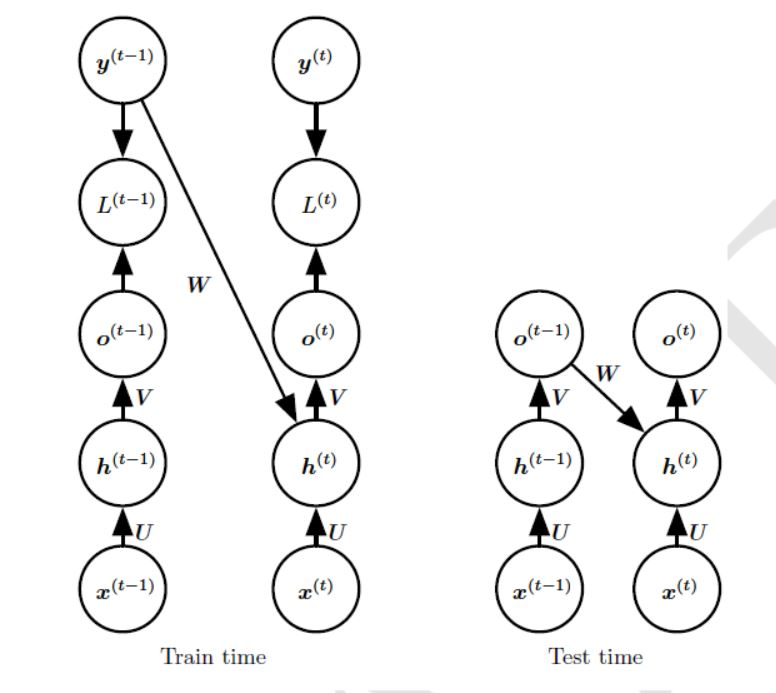
\includegraphics[width=0.8\textwidth]{f6}
                \caption{导师驱动过程的示意图。导师驱动过程是一种训练技术,适用于输出与下一时间步的隐藏状态存在连接的RNN。(左)训练时,我们将训练集正确的输出$y^{(t)}$反馈到$h^{(t+1)}$。(右)当模型部署后,真正的输出通常是未知的。在这种情况下,我们用模型的输出$o^{t}$来近似正确的输出$y^{(t)}$,并反馈回模型}
                \label{f10.6}
            \end{figure}
            如果之后网络在\textbf{开环(Open-loop)}模式下使用,即网络输出反馈作为输入,那么完全使用导师驱动过程进行训练的缺点就会出现。在这种情况下,训练期间该网络看到的输入和测试时看到的会有很大的不同,减轻此问题的一种方法是同时使用导师驱动过程和自由运行的输入进行训练,例如在展开循环的输出到输入路径上预测几个步骤的正确目标值。通过这种方式,网络可以学会在训练时没有接触到的输入条件,以及将状态映射回使网络几步之后生成正确输出的状态。另一种方式是通过随意选择生成指或者真实数据值作为输入以减小训练时和测试时看到的输入之间的差别,这种方法利用了课程学习策略,逐步使用更多生成值作为输入。

        \subsection{计算循环神经网络的梯度}
            计算循环神经网络的梯度是很容易的。我们可以将之前推广的反向传播算法应用于展开的计算图中。而不需要特殊化的算法。由反向传播计算得到的梯度,并结合任何通用的基于梯度的技术就可以训练RNN。

            为了获得BPTT算法行为的一些直观理解,我们举例说明如何通过BPTT计算上述RNN公式\ref{e10.8}和公式\ref{e10.12}的梯度。计算图的节点包括参数$U,V,W,b,c$以及以时间$t$为索引的节点序列$x^{(t)},h^{(t)},o^{(t)},L^{(t)}$。对于每一个节点$\textbf{N}$,我们需要基于$\textbf{N}$后面的节点的梯度。递归地计算梯度$\nabla_N L$。我们从紧接着最终损失的节点可以递归:
            \begin{equation}
                \frac{\partial L}{\partial L^{(t)}} = 1
                \label{e10.17}
            \end{equation}
            这个导数中,假设输出$o^{(t)}$作为softmax函数的参数,我们可以从softmax函数获得关于输出概率的向量$\hat{y}$。我们也假设损失是迄今为止给定了输入后的真实目标$y^{(t)}$的负对数似然。对于所有的$i,t$,关于时间步$t$输出的梯度$\nabla_{o^{(t)}} L$ 如下:
            \begin{equation}
                (\nabla_{o^{(t)}} L)_i = \frac{\partial L}{\partial o_i^{(t)}} = \frac{\partial L}{\partial L^{(t)}} \frac{\partial L^{(t)}}{\partial o_i^{(t)}} = \hat{y}_i^{(t)} - 1_{i,y^{(t)}}
                \label{e10.18}
            \end{equation}
            我们从序列的末尾开始,反向计算。在最后的时间步$\tau$,$h^{(\tau)}$只有$o^{(\tau)}$作为后续节点,因此这个梯度很简单:
            \begin{equation}
                \nabla_{h^{(\tau)}} L = V^T \nabla_{o^{(\tau)}} L
                \label{e10.19}
            \end{equation}
            然后,我们可以从时刻$t=\tau-1$到$t=1$反向迭代,通过时间反向传播梯度,注意$h^{(t)}(t<\tau)$同时具有$o^{(t)}$和$h^{(t+1)}$两个后续节点。因此它的梯度由下列公式计算
            \begin{equation}
                \begin{split}
                    \nabla_{h^{(t)}} L &= (\frac{\partial h^{(t+1)}}{\partial h^{(t)}})^T (\nabla_{h^{(t+1)}} L) + (\frac{\partial o^{(t)}}{\partial h^{(t)}})^T(\nabla_{o^{(t)}}L) \\
                    &=W^T(\nabla_{h^{(t+1)}}L) diag(1-(h^{(t+1)})^2) + V^T(\nabla_{o^{(t)}} L)
                \end{split}
                \label{e10.20}
            \end{equation}
            其中$diag(1-(h^{(t+1)})^2)$表示包含元素$1-(h_i^{(t+1)})^2$的对角矩阵。这是关于时刻$t+1$与隐藏单元$i$关联的双曲正切的Jacobian矩阵。

            一旦获得了计算图内部节点的梯度,我们就可以得到关于参数节点的梯度。因为参数在许多时间步上共享,我们必须在表示这些变量的微积分操作时谨慎对待。我们希望实现的是等式计算计算图中单一边对梯度的贡献。然而微积分中的$\nabla_W f$算子,计算$W$对于$f$的贡献时将计算图中所有的边都考虑进去了。为了消除这种歧义,我们定义只在$t$时刻使用的虚拟变量$W^{(t)}$作为$W$的副本。然后,可以使用$\nabla_{W^{(t)}}$表示权重在时间步$t$对梯度的贡献。

            使用这个表示,关于剩下参数的梯度可由下列公式给出:
            \begin{align}
                    \nabla_c L &= \sum_t (\frac{\partial o^{(t)}}{\partial c})^T \nabla_{o^{(t)}} L = \sum_t \nabla_{(o^{(t)})} L \\
                    \nabla_b L &= \sum_t (\frac{\partial h^{(t)}}{\partial b}) = \sum_{t} diag(1-(h^{(t)})^2) \nabla_{h^{(t)}} L \\
                    \nabla_V L &= \sum_t\sum_i(\frac{\partial L}{\partial o_i^{t}}) \nabla_V o_i^{(t)} = \sum_t (\nabla_o^{(t)}L)h^{(t)^T} \\
                    \nabla_W L & = \sum_t\sum_i(\frac{\partial L}{\partial h_i^{(t)}})\nabla_{W^{(t)}} h_i^{(t)}=\sum_t diag(1-(h^{(t)})^2)(\nabla_{h^{(t)}}L)h^{(t-1)^T} \\
                    \nabla_U L &= \sum_t\sum_i (\frac{\partial L}{\partial h_i^{(t)}})\nabla_{U^{(t)}}h_i^{(t)} = \sum_t diag(1-(h^{(t)})^2) (\nabla_{h^{(t)}}L)x^{(t)^T}
            \end{align}
            因为计算图中定义的损失的任何参数都不是训练数据$x^{(t)}$的父节点,所以我们不需要计算关于它的梯度。

        \subsection{作为有向图模型的循环网络}
            目前为止,我们接触的循环网络例子中损失$L^{(t)}$是训练目标$y^{(t)}$和输出$o^{(t)}$之间的交叉熵。与前馈网络类似,原则上循环网络几乎可以使用任何损失。但必须根据任务来选择损失。如前馈网络,通常我们希望将RNN的输出解释为一个概率分布,并且通常使用与分布相关联的交叉熵来定义损失。均方误差是与单位高斯分布的输出想关联的交叉熵,例如前馈网络中所使用的。当使用一个预测性对数似然的训练目标,如公式\ref{e10.12},我们将RNN训练为能够根据之前的输入估计下一个序列元素$y^{(t)}$的条件分布。这可能意味着,我们最大化对数似然
            \begin{equation}
                \log P(y^{(t)}|x^{(1)},\cdots,x^{(t)})
                \label{e10.29}
            \end{equation}
            或者,如果模型包括来自一个时间步的输出到下一个时间步的连接,则为如下形式
            \begin{equation}
                \log P(y^{(t)}|x^{(1)},\cdots,x^{(t)},y^{(1)},\cdots,y^{(t-1)})
                \label{e10.30}
            \end{equation}
            将整个序列$y$的联合分布分解为一系列单步的概率预测是捕获关于整个序列完整联合分布的一种方法。如果我们不把过去的$y$值反馈给下一步作为预测的条件,那么有向图模型不包括任何从过去$y^{(i)}$到当前$y^{(t)}$的边。这种情况下,输出$y$和给定的$x$序列是条件独立的。如果我们反馈真实的$y$值给网络,那么有向图模型包含所有从过去$y^{(i)}$到当前$y^{(t)}$的边。

            举一个例子,让我们考虑对标量随机变量序列$\mathbb{Y}=\{y^{(1)},\cdots,y^{(\tau)}\}$建模的RNN,也没有额外的输入$x$。在时间步$t$的输入仅仅是时间步$t-1$的输出。该RNN定义了关于$y$变量的有向图模型。我们使用链式法则参数化这些观察值的联合分布:
            \begin{equation}
                P(\mathbb{Y}) = P(y^{(1)},\cdots,y^{(\tau)}) = \prod_{t=1}^{\tau} P(y^{(t)}|y^{(t-1)},\cdots,y^{(1)})
                \label{e10.31}
            \end{equation}
            因此,根据这样一个模型,一组值$\{y^{(1)},\cdots,y^{(\tau)}\}$的负对数似然为
            \begin{equation}
                L = \sum_t L^{(t)}
                \label{e10.32}
            \end{equation}
            其中
            \begin{equation}
                L^{(t)} = -\log P(y^{(t)}|y^{(t-1)},\cdots,y^{(1)})
                \label{e10.33}
            \end{equation}
            图模型中的边表示哪些变量直接依赖于其他变量。许多图模型的目标是省略不存在强相互作用的边以实现统计和计算的效率。例如,我们通常可以做Markov假设,即图模型应该只依赖于有限期历史数据而不是整个历史数据。然后,在一些情况下,我们认为整个过去的输入会对序列的下一个元素有一定的影响。当我们认为$y^{(t)}$的分布可能取决于遥远过去的$y^{(i)}$的值,且无法通过$y^{(t-1)}$捕获$y^{(i)}$的影响时,RNN 将会很有用。

            解释RNN作为图模型的一种方法是将RNN视为定义一个结构为完全图的图模型,且能够表示任何一对$y$值之间的直接联系。图\ref{f10.7}是关于$y$值且具有完全图结构的图模型。该RNN完全图的解释基于排除并忽略模型中的隐藏单元$h^{(t)}$。
            \begin{figure}[h]
                \centering
                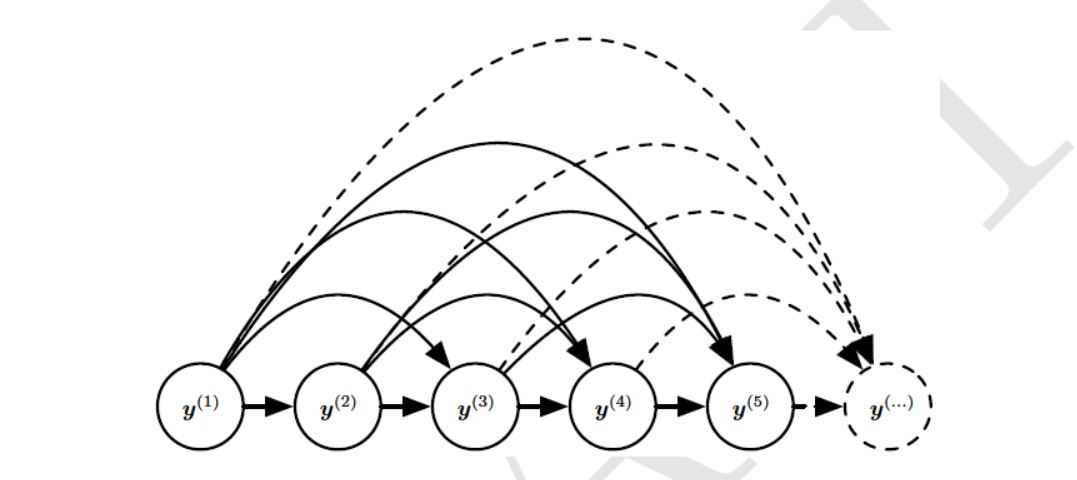
\includegraphics[width=0.8\textwidth]{f7}
                \caption{序列$y^{(1)},y^{(2)},\cdots,y^{(t)}$的全连接图模型。给定先前的值,每个过去的观察值$y^{(i)}$可以影响后续节点的条件分布。当序列中每个元素的输入和参数的数目越来越多,根据此图直接参数化图模型可能是非常低效的。RNN可以通过高效的参数化获得相同的全连接}
                \label{f10.7}
            \end{figure}

            更有趣的是,将隐藏单元$h^{(t)}$视为随机变量,从而产生RNN的图模型结构。在图模型中包含隐藏单元预示RNN能对观测的联合分布提供非常有效的参数化。假设我们用表格表示法来表示离散值上的任意的联合分布,即对每个值可能的赋值分配一个单独条目的数组,该条目表示发生该赋值的概率。如果$y$可以取$k$个不同的值,表格表示法将有$\mathcal{O}(k^{(\tau)})$个参数。对比RNN,由于参数共享,RNN的参数数目为$\mathcal{O}(1)$且是序列长度的函数。我们可以调节RNN的参数数量来控制模型容量,但不用被迫于序列长度成比例。公式\ref{e10.5}展示了所述的RNN通过循环应用相同的函数$f$以及在每一个时间步的相同参数$\theta$,有效地参数化的变量之间的长期联系。图\ref{f10.8}说明了这个图模型的解释。在图模型中结合$h^{(t)}$节点可以用作过去和未来之间的中间量,从而将它们解耦。遥远过去的变量可以通过隐藏变量来影响未来的变量。该图的结构表明可以在时间步使用相同的条件概率分布有效地参数化模型,并且当观察到全部变量时,可以高效地评估联合分配给所有变量的概率。

            即便使用高效参数化的图模型,某些操作在计算上仍然具有挑战性。例如,难以预测序列中缺少的值。

            循环网络为了减少的参数数目付出的代价是优化参数可能变得困难。

            在循环网络中使用的参数共享的前提是相同参数可用于不同时间步的假设。也就是说,假设给定时刻$t$的变量后,时刻$t+1$变量的条件概率分布是平稳的,这意味着之前的时间步和下个时间步之间的关系并不依赖于$t$。原则上,可以使用$t$作为每个时间步的额外输入,并让学习其在发现任何时间依赖性的同时,也在不同时间步之间尽可能多地共享。相比在每个$t$使用不同的条件概率分布已经好多了,但网络将必须在面对新$t$时进行推断。
            \begin{figure}[h]
                \centering
                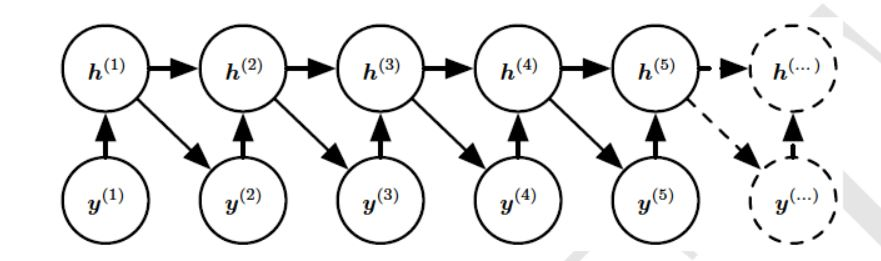
\includegraphics[width=0.8\textwidth]{f8}
                \caption{在RNN图模型中引入状态变量,尽管它是输入的确定性函数,但它有助于我们根据公式\ref{e10.5}获得非常高效的参数化。序列中的每个阶段都使用相同的结构,并且可以与其他阶段共享参数}
                \label{f10.8}
            \end{figure}
            为了完整描述将RNN作为图模型的观点,我们必须描述如何从模型中进行采样。我们需要执行的主要操作是简单地从每一时间步的条件分布中采样。然而,这会导致额外的复杂性。RNN必须有某种机制来确定序列的长度。这可以通过多种方式来确定。
            
            在当输出是从词汇表获取的符号的情况下,我们可以添加一个对应于序列末端的特殊符号。当产生该符号的时候,采样过程停止。





\end{document}

